\documentclass{scrartcl}
\usepackage{style}
\usepackage{float}
% version
\newcommand{\versionmajor}{0}
\newcommand{\versionminor}{1}
\newcommand{\versionpatch}{0}
\newcommand{\version}{\versionmajor.\versionminor.\versionpatch}

\title{\LARGE
    % Final Report Template
    Study and Implementation of the Sieve Protocol in BFT
}

% \subtitle{(v. \version)}

% Consider watching:
% https://www.youtube.com/watch?v=ihxSUsJB_14
% https://www.youtube.com/watch?v=XTFWaV55uDo

\author{
    Samuele De Tuglie \\ \emailaddr{samuele.detuglie@studio.unibo.it}
    \and 
    Emanuele Artegiani \\ \emailaddr{emanuele.artegiani@studio.unibo.it} 
    \and 
    Pablo Sebastian Vargas Grateron \\ \emailaddr{pablo.vargasgrateron@studio.unibo.it}
}

\date{\today}

\begin{document}

\maketitle

\begin{abstract}
This project aims to create a simulation of the Sieve protocol for Byzantine Fault Tolerance (BFT). Establishing a resilient and dependable replicated state machine (RSM) that can tolerate Byzantine faults in a distributed network was the main goal. During the simulation process, it is important to guarantee scalability and effective resource management. Furthermore, we offer a basic client that can communicate with the RSM by performing a small set of actions.

To evaluate the resilience of the protocol, Byzantine actors are included in the simulation, which comprises numerous nodes, each of which represents a participant in the RSM. Identifying and alleviating Byzantine faults by putting the Sieve protocol into practice will protect the distributed system's integrity and consistency even when there are malicious nodes present.

In order to prevent Byzantine failures, the Sieve protocol requires at least \textit{3f + 1} nodes, where \textit{f} is the number of faulty ones.

The simulation's outcomes show how well the Sieve process works to achieve BFT. This project offers a basic, user-friendly tool for experimentation and analysis, advancing our understanding of and ability to apply Byzantine fault-tolerant protocols in distributed systems.
\end{abstract}


\newpage


\section{Goals/Requirements}

\subsection{Project Goals}

The primary goals of this project include:

\begin{itemize}
    \item \textbf{Implementation of Sieve Protocol}
    
    To improve the resilience of distributed systems, create a working simulation of the Sieve protocol with a focus on BFT.

    \item \textbf{Use of Consensus}

    Create an RSM, that acts as a server, wherein consensus is used to make decisions.

    \item \textbf{Concurrent Programming}

    Utilize numerous threads to run several routines concurrently.
    
    \item \textbf{Docker Integration}
    
    For containerization, use Docker to guarantee scalable deployment and effective resource management during the simulation process.

    \item \textbf{Graphical User Interface (GUI)}
    
    Provide a user-friendly graphical user interface (GUI) that offers centralized control over the simulation. Due to the project's simulation goal, it ought to have a \textit{Admin} section and a \textit{Client} section in the same GUI.

    \item \textbf{Scalability Analysis}
    
    Assess the system's scalability under varying conditions to understand the protocol's effectiveness in maintaining fault tolerance.

    \item \textbf{Automated Testing}
    
    Include automated tests to verify that the functionalities are correct.
\end{itemize}


\subsection{Project requirements}

The requirements of this project include:

\begin{itemize}
    \item \textbf{Architectural Requirements}

    Internal communication among RSM nodes and between them and clients will be based on the UDP protocol.

    \item \textbf{Simulation Requirements}

    The Sieve protocol can manage \textit{f} Byzantine nodes out a total of \textit{3f + 1}. To simulate a Byzantine behavior we will set \textit{f} faulty nodes artificially.

    \item \textbf{Functionalities}

    A basic key-value store database is the primary feature of the RSM. Clients have the ability to add, modify, and get values in the database. Since the project's main goal is to achieve the BFT via the Sieve protocol, just these bare minimum operations will be carried out.


\end{itemize}

\subsection{Expected Outcomes}

Upon completion, the project is expected to yield the following principal outcomes:

\begin{itemize}
    \item \textbf{Functional Simulation}

    A fully functional simulation of the Sieve protocol with integrated BFT mechanisms and consensus.

    \item \textbf{Dockerized Deployment}

    Docker containers are configured for each node, facilitating easy deployment, scalability, and resource management.

    \item \textbf{Intuitive GUI}

    A user-friendly GUI lets users interact with the RSM.
    
\end{itemize}

\subsection{Use Case Diagram}

The use case diagram \ref{fig:use-cases} illustrates the interactions and functionalities of the Sieve protocol simulation. These visual representations serve as valuable references for understanding the roles and responsibilities of each entity in the system.

\begin{figure}[H]
    \centering
    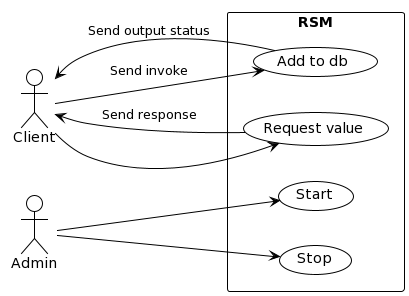
\includegraphics[width=.6\linewidth]{figures/use-cases.png}
    \caption{Use case diagram representing the interaction between admin/client and RSM.}
    \label{fig:use-cases} 
\end{figure}


\subsection{Scenarios}

Users are expected to interact with the project through the GUI, employing some functionalities to manage and interact with the Sieve protocol simulation. The following scenarios outline how and why users would engage with the system:

\subsubsection{Admin}

\begin{enumerate}
    \item \textbf{Start and Stop Docker Containers}
        \begin{itemize}
            \item \textit{How:} Admins can initiate and terminate Docker containers through the GUI.
            \item \textit{Why:} This functionality provides admins with control over the simulation life-cycle, allowing them to start and stop the RSM.
        \end{itemize}
\end{enumerate}

\subsubsection{Client}

\begin{enumerate}
    \item \textbf{Add items to database}
        \begin{itemize}
            \item \textit{How:} Users can input and send data through the GUI to be added to the RSM database.
            \item \textit{Why:} This scenario enables users to dynamically influence the data synchronized among the nodes, simulating real-world scenarios where key updates or additions occur.
        \end{itemize}

    \item \textbf{Request item from database}
        \begin{itemize}
            \item \textit{How:} Users can input the key of the item requested in the GUI.
            \item \textit{Why:} This scenario enables users to dynamically request the value associated with the key inserted, simulating real-world scenarios.
        \end{itemize}
    \item \textbf{Check Incoming Messages}
        \begin{itemize}
            \item \textit{How:} Users can use the GUI to monitor incoming messages to each node in real-time.
            \item \textit{Why:} To make it easier to spot unusual behavior and abnormalities, this feature enables users to view the distributed system's output messages as well as log messages that it generates.
        \end{itemize}
        
\end{enumerate}

These scenarios collectively empower users to interact with the project in a controlled, fostering experimentation, analysis, and a deeper understanding of Byzantine fault-tolerant protocols in distributed systems.


\subsection{Self-assessment policy}

\begin{itemize}
    \item \textbf{Assessment of Software Quality}
    
    The quality of the produced software will be assessed through the following criteria:
    \begin{itemize}
        \item \textit{Automated Testing:} The software includes a comprehensive suite of automated tests implemented using the Python \textit{unittest} framework. These tests cover various aspects of the codebase, ensuring functionality, reliability, and adherence to specifications.
        
        \item \textit{Code Maintainability:} The project code follows best practices for readability, maintainability, and documentation. The creation of modular code with thorough comments and documentation makes it easy to maintain and comprehend due to its breakdown into related components.
    
        \item \textit{Scalability and Performance:} The software undergoes testing for scalability and performance under various conditions, ensuring it meets the specified requirements and performs well in different scenarios.

        \item \textit{Reliability:} Measured in terms of fault tolerance.

        \item \textit{Communication Security:} All the communications are encrypted to enhance security.
    \end{itemize}

    \item \textbf{Assessment of Project Outcomes' Effectiveness}
    
    The effectiveness of the project outcomes will be evaluated based on the following criteria:
    \begin{itemize}
        \item \textit{Protocol Functionality:} The successful implementation and functionality of the Sieve protocol in Byzantine fault-tolerant scenarios will be a key factor in assessing the project's effectiveness.
        
        \item \textit{User Interaction:} The usability of the GUI and its ability to provide users with intuitive interaction with the RSM.
        
        \item \textit{Simulation Results:} The project's effectiveness will be gauged by the analysis of simulation results, including the detection and mitigation of Byzantine faults, scalability insights, and overall system performance.
        
        \item \textit{Documentation:} The clarity and completeness of project documentation, including user guides, code documentation, and system architecture, contribute to the overall assessment of project outcomes.
    \end{itemize}
\end{itemize}

\newpage

\section{Background}

To comprehend the essence and rationale of this project, it is imperative to explore its theoretical foundation. At the heart of this initiative lies the implementation of the Sieve protocol, a cutting-edge approach to achieving BFT expounded in the referenced paper \cite{paper}.

State-machine replication enhances application resilience by executing it across multiple independent components, employing BFT to ensure consistency. BFT enables correct outputs with a majority of processes being correct, even in the presence of adversarial behavior. However, traditional replication assumes determinism, posing challenges for non-deterministic applications like those involving cryptography. The work introduces two protocols: \textit{Sieve}, which detects and handles minor divergences among processes, and Mastercrypt, providing cryptographic security for random functions in master-slave replication. These protocols aim to address non-determinism in BFT replication, crucial for applications like permissioned blockchains.

When the application cannot be altered, modular replicated execution becomes necessary, often the practical scenario. Two integration approaches exist: \textit{order-then-execute} orders operations before independent execution, communicating results via atomic broadcast, ensuring deterministic steps. Alternatively, \textit{execute-then-order} executes operations speculatively first, then agrees on the output, possibly rolling back diverging results. Protocol Sieve, introduced here, utilizes speculative execution, adhering to execute-then-order. It's tailored for occasionally non-deterministic applications, offering a modular solution for replicating them within a BFT system.

The system comprises distributed processes\footnote{Processes and nodes in this paper are used equivalently and with the same meaning.} providing a fault-tolerant service via service replication. Processes communicate via broadcast, executing requests in the same order. Non-faulty processes are termed correct, while faulty processes may crash or exhibit Byzantine faults. Protocols are presented modularly, using event-based notation, with processes defined by interfaces and properties. Authenticated point-to-point communication ensures message integrity via shared secret keys. The system is partially synchronous, allowing unbounded message delays until eventual synchronization, representing real-world network scenarios.

In a broadcast primitive involving \textit{n} processes, messages are broadcast and delivered upon agreement. The atomic broadcast also tackles the consensus problem, with a variant ensuring the delivery of messages satisfying an external validity condition. The definition of Byzantine atomic broadcast with external validity involves input and output events, governed by a validation predicate ensuring correct message delivery based on local computation by each process.

An RSM executes operations and maintains a consistent state across correct processes. Defined by input and output events, it guarantees agreement, correctness, and termination properties. The standard implementation relies on the atomic broadcast to disseminate requests, ensuring all processes start from the same initial state and execute operations in the delivered order. If operations are deterministic, correct processes' states remain consistent.

In the context of atomic broadcast implementations, synchrony assumptions or randomization are often necessary. An eventual leader-detector oracle is a common weak timing assumption, informing processes of a correct leader to facilitate protocol progress. For Byzantine processes, a leader detector can be implemented from a failure detector, albeit with more complexity due to arbitrary behavior. Processes employ a "trust, but verify" approach to monitor leader behavior, initiating leader switches upon detection of misbehavior. Byzantine leader detectors and epoch-change primitives ensure trust, agreement, and resistance to coups in leader elections, while also ensuring eventual leadership among correct processes. Cryptographic functionalities, such as hash functions and digital signature schemes, are modeled as ideal, deterministic functionalities implemented by distributed oracles, ensuring collision resistance and signature verification properties.

\textit{Protocol Sieve} operates within a Byzantine atomic broadcast framework with weak external validity and employs a \textit{Sieve-leader} for executing non-deterministic operations. The leader is elected using a Byzantine epoch-change abstraction, ensuring configurations progress with monotonically increasing epoch numbers. Each configuration has its Sieve-leader, to whom all operations are sent via an INVOKE message. Operations are executed speculatively, and the leader confirms them upon receiving 2f + 1 APPROVE messages from distinct processes. The confirmed operation is then broadcasted for commitment. Sieve ensures consensus on leader changes via atomic broadcast, preventing denial-of-service attacks and ensuring liveness. Sieve's design mitigates uncoordinated speculative request execution to prevent contention among self-proclaimed leaders, crucial for maintaining liveness in BFT protocols. While a faulty leader could disrupt liveness, this is consistent with other leader-based BFT protocols. The protocol's implementation details assume authenticated, unforgeable, FIFO-ordered point-to-point messages among correct processes, with unique invoked operations across all processes.


Optimizations Rollback and state transfer in Protocol Sieve ensure efficient recovery of application states post-operation. By utilizing rollback and state transfer primitives, processes can efficiently recover correct states from other clients, minimizing overhead. Additionally, synchronization with PBFT-based atomic broadcast further enhances efficiency, leveraging PBFT's leader and Byzantine epoch-change mechanisms for seamless integration with Sieve. These optimizations minimize message overhead while ensuring consistent state recovery and operation execution.

It should be noted that Sieve not only works with Byzantine atomic broadcast in the model of eventual
synchrony but can equally well be run over randomized Byzantine consensus.\\


\subsection{Used Frameworks / Models / Technologies}
    
The development of this project is centered around the Python programming language, chosen for its versatility and extensive libraries that facilitate rapid application development. Specifically, the following frameworks, models, and technologies were employed:

\begin{itemize}
    \item \textbf{Python}
    
    The entire project, including the Sieve protocol implementation, GUI development, and automated testing, is written in \textit{Python}. Its readability, flexibility, and vast community support make it suitable for this endeavor.
    
    \item \textbf{PySimpleGUI}
    
    The GUI is constructed using \textit{PySimpleGUI}, a Python GUI framework. Its simplicity and ease of use align with the project's goal of providing an intuitive interface for users to interact with the simulation.
    
    \item \textbf{unittest}
    
    Automated testing is facilitated through the use of the \textit{unittest} framework in Python. This allows for the systematic testing of individual components, ensuring code reliability and functionality.
    
    \item \textbf{Docker}
    
    \textit{Docker} is utilized for containerization, providing a lightweight and portable environment for the Sieve protocol simulation. Docker-Compose is employed to manage the orchestration of multiple containers, streamlining the deployment process and ensuring consistency across different environments.
\end{itemize}

The choice of these technologies is motivated by their compatibility, community support, and ability to enhance the overall development and deployment process of the Sieve protocol simulation.

% \section{Design}

% This is where the logical / abstract contribution of the project is presented.

% Notice that, when describing a software project, three dimensions need to be taken into account: structure, behavior, and interaction.

% Always remember to report \textbf{why} a particular design has been chosen.
% Reporting wrong design choices that have been evaluated during the design phase is welcome too.
\section{Requirements Analysis}

The functional requirements of the application encompass all the features and services provided by the system:

\begin{itemize}
    \item \textbf{Start and Stop Docker Container}
    
    Initiate and terminate the Docker container seamlessly, ensuring a controlled environment for the Sieve protocol simulation.
    \item \textbf{Data Management}
    
    Enable the transmission of data to individual nodes, facilitating dynamic adjustments to their behaviors and configurations during the simulation.
    \item \textbf{Shared Data Retrieval}
    
    Facilitate the retrieval of shared data between nodes, essential for evaluating the consensus achieved by the Sieve protocol in the presence of Byzantine faults.
    \item \textbf{Log Inspection}
    
    Provide a mechanism to inspect the log of messages from the RSM, aiding in debugging, analysis, and a comprehensive understanding of the simulation's dynamics.
\end{itemize}

\subsection{Implicit Requirements}

Implicit requirements, not explicitly defined above but nevertheless fundamental, include:

\begin{itemize}
    \item \textbf{Compatibility}
    
    The software is designed to function on every platform where Docker and Python are runnable, ensuring compatibility with almost every modern device.
    \item \textbf{Software Functionality Testing}
    
    Various tests are embedded in the program to ensure the correct functionality of the code.
\end{itemize}

\subsection{Non-Functional Requirements}

Non-functional requirements express the characteristics and properties that a system must meet. The following non-functional requirements are present in the project:

\begin{itemize}
    \item \textbf{Scalability}
    
    Each node is represented by a Docker container, facilitating network expansion by simply adding new nodes to the Docker Compose file.
    \item \textbf{Security}
    
    As indicated in \cite{paper}, the software utilizes symmetric cryptography to encrypt and decrypt messages, ensuring the confidentiality and integrity of communication.
    \item \textbf{Usability}
    
    The software is equipped with a user-friendly dashboard to interact with the nodes, enhancing the overall user experience.
    \item \textbf{Maintainability}
    
    The code has been crafted clearly, simply, and understandable, ensuring ease of maintenance and future enhancements.
\end{itemize}


\subsection{Implicit Assumptions}

Some implicit assumptions are noteworthy as they influence the design of the system:

\begin{itemize}
    \item \textbf{Ports Not Occupied}
    
    Each Docker container runs and exposes a port. It is essential to check if the port to use is unoccupied.
    
    \item \textbf{Administrator Presence}
    
    It is assumed that there is a system administrator familiar with the IP addresses and ports made available by each node for the protocol implementation. In our simulation, this role is fulfilled using the \emph{client\_config.py} file.
    
    \item \textbf{Number of Nodes}
    
    Two potential issues may arise when a node experiences Byzantine faults. The first problem is the failure to send a message altogether. Specifically, within a distributed system to function correctly with \(N\) nodes, having \(f\) nodes suffering from Byzantine faults, consensus must be reached with \(N - f\) messages. In other words, \(N - f\) nodes are required for the quorum. 

    The second problem arises when a Byzantine-faulty node maliciously sends different messages. In an extreme scenario, let's say that among the \(N - f\) nodes that have achieved quorum, \(f\) have been sent by a Byzantine-faulty node. Even in this case, the system must operate normally, requiring \((N - f) - f\) messages to be greater than \(f\) messages sent by nodes experiencing Byzantine faults. To solve the two aforementioned problems, \((N - f) - f > f\). Therefore, in a BFT system, the total number of processes must be \(3f + 1\) to tolerate \(f\) faulty nodes.
    
\end{itemize}

\subsection{Models/Paradigms/Technologies}

Among the models, paradigms, and technologies best suited to address the previously mentioned requirements are:

\begin{itemize}
    \item \textbf{Client-Server Architectural Paradigm}
    
    The client communicates with the server using UDP protocol.
    \item \textbf{Master-Slave Model}
    
    Inside the server, a master-slave model is employed.
\end{itemize}



\subsection{Structure / Domain Entities}
To gain a comprehensive understanding of the entities requiring modeling, reference the UML class diagram depicted in Figure~\ref{fig:classes}. Method and variable names defined in the reference paper \cite{paper} were retained as much as possible.

\begin{figure}[H]
    \centering
    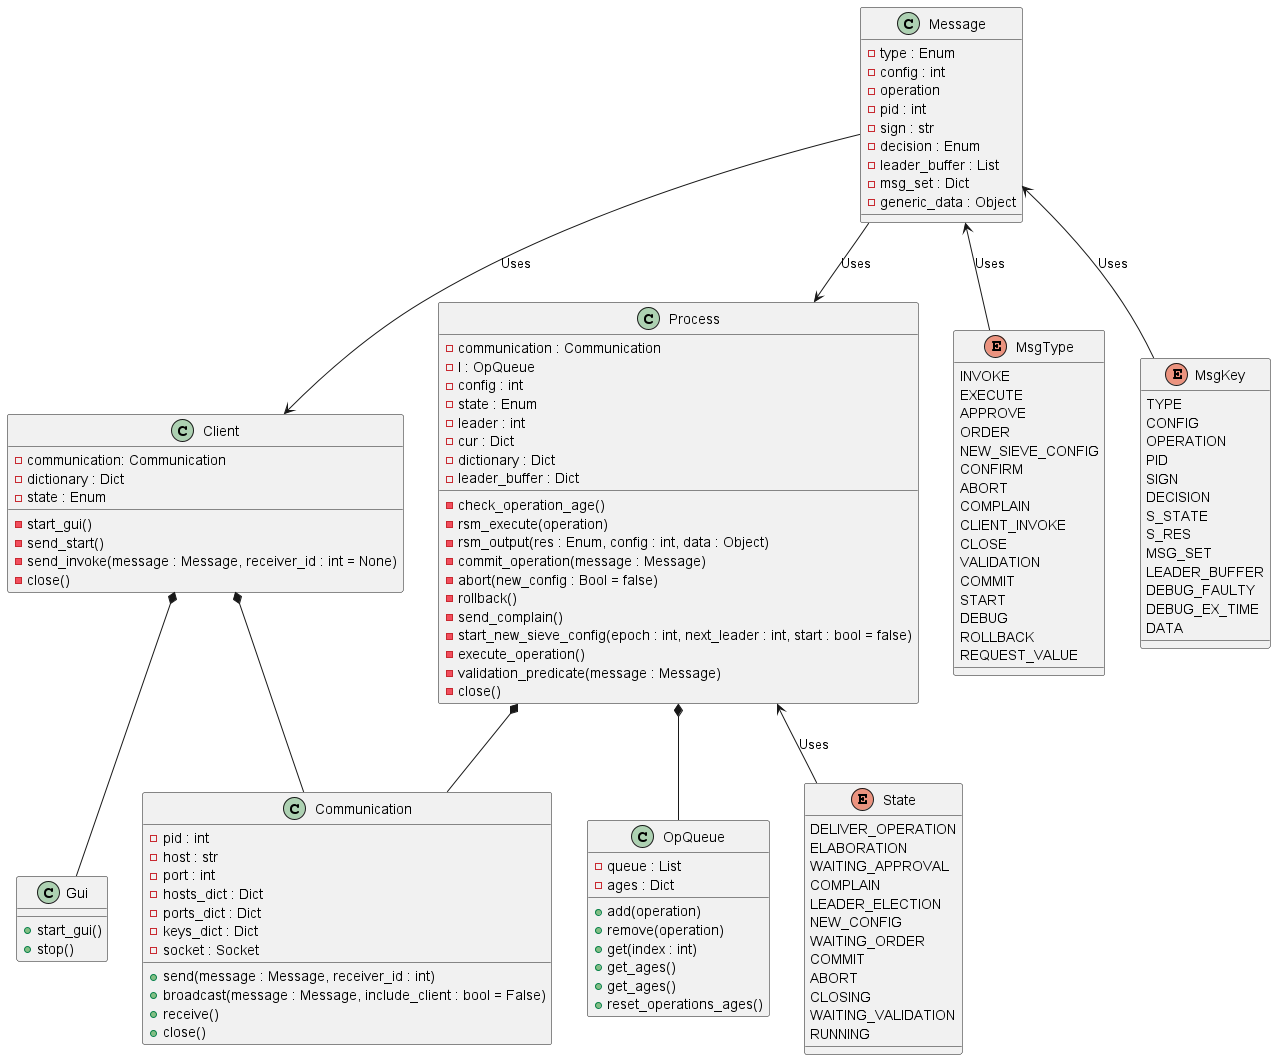
\includegraphics[width=1\linewidth]{figures/classes.png}
    \caption{Class Diagram}
    \label{fig:classes} 
\end{figure}

This diagram represents the following domain entities:

\begin{itemize}
    \item \textbf{Process:} A class representing the Sieve protocol node.
    \item \textbf{Message:} A data class that encapsulates the attributes of a message.
    \item \textbf{Client:} A class responsible for controlling interactions from the client to the server.
    \item \textbf{Communication:} A class designed to handle the exchange of messages.
    \item \textbf{Gui:} A class managing the user interface components.
    \item \textbf{OpQueue:} A class for queuing up operation requests initiated by the client.
    \item \textbf{State:} An enumeration representing the various states of the Sieve nodes.
    \item \textbf{MsgType:} An enumeration declaring different types of messages.
    \item \textbf{MsgKey:} An enumeration is used to compose the messages.
\end{itemize}


\subsection{Behaviour}

\subsubsection{Leader node}

% How should each entity behave?
%
% (UML State diagram or Activity Diagram)
% PROBABLY ADD UML MADE BY US

% \subsection{Interaction}

% How should entities interact with each other?
% %
% (UML Sequence Diagram)
The leader node in the Sieve Protocol exhibits the following behavior (as expressed in the figure \ref{fig:leader}):
\begin{figure}[H]
    \centering
    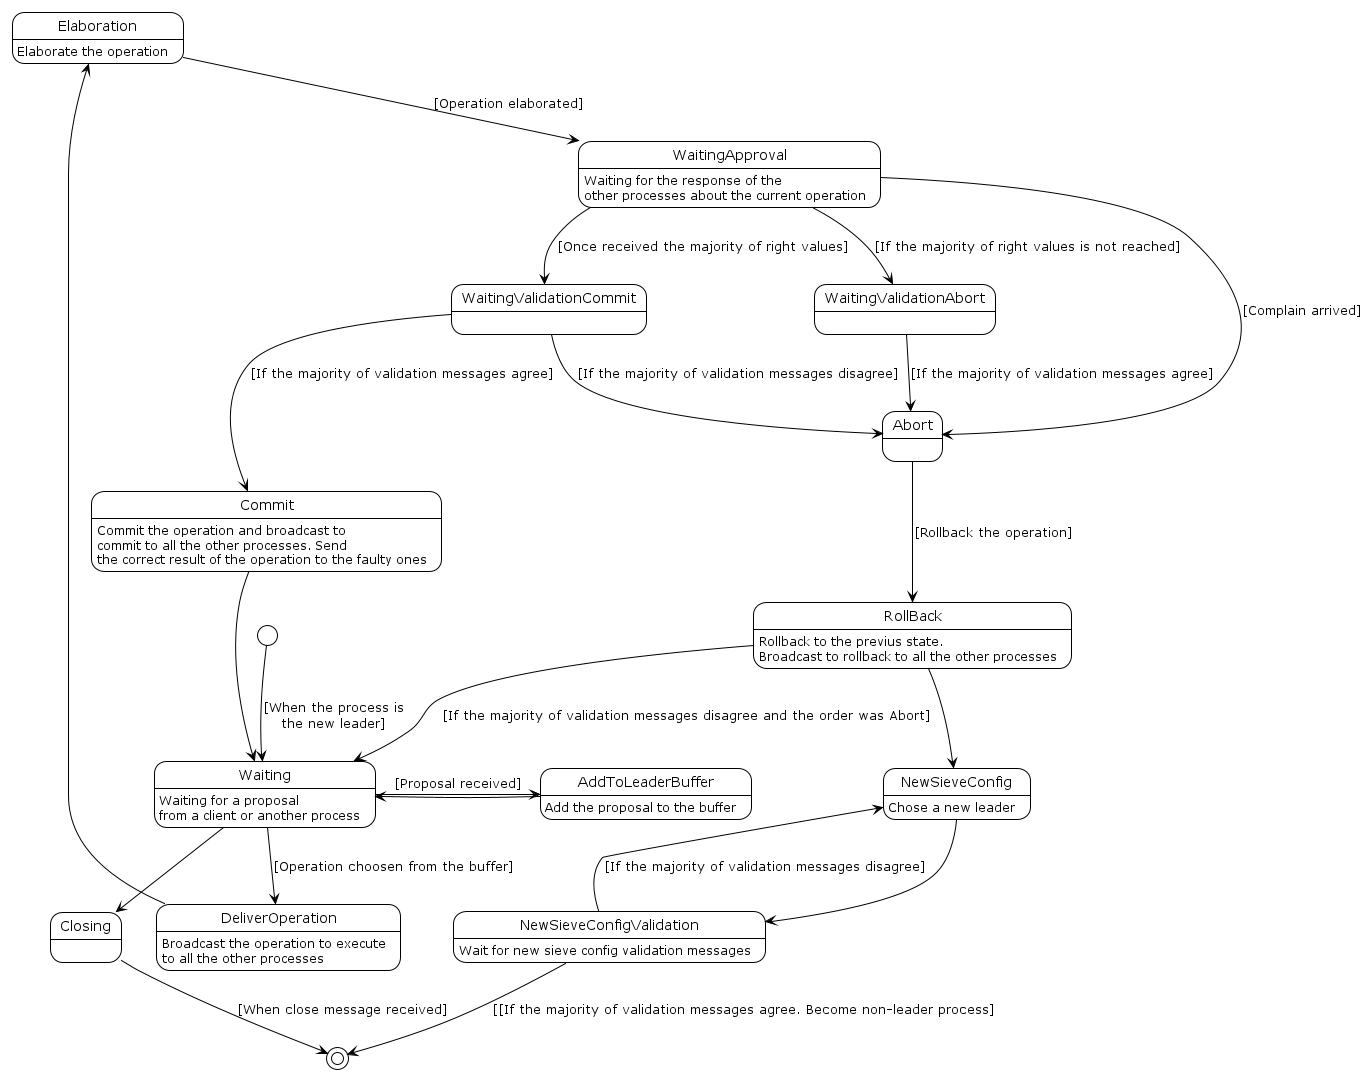
\includegraphics[width=1\linewidth]{figures/leader.png}
    \caption{State diagram of leader node}
    \label{fig:leader} 
\end{figure}

\begin{itemize}
    \item \textbf{Waiting}
    
    This is the idle status, during which the leader awaits further operations to be requested from a client or another process.

    \item \textbf{AddToLeaderBuffer}
    
    During this state, the leader adds the requested operation to its buffer for processing.
    
    \item \textbf{DeliverOperation}
    
    When an operation is requested, the leader broadcasts the operation to be executed to all other processes in the network.
    
    \item \textbf{Elaboration}
    
    The leader processes the requested operation. If the leader receives a complaint message from any slave during this state, it transitions to the \textbf{Abort} state and then to \textbf{NewSieveConfig}.
    
    \item \textbf{WaitingApproval}
    
    After completing the operation, the leader broadcasts the local result and waits for confirmation from at least \(2f+1\) processes. Also in this state if the leader receives a complaint message from any slave during this state, it transitions to the \textbf{Abort} state and then to \textbf{NewSieveConfig}.
    
    \begin{itemize}
        \item \textit{WaitingValidationCommit}
        
        If the majority of processes validate the leader's result, the leader enters this state, awaiting validation of its local result from the majority of processes. If the majority validates the result, the state transitions to \textbf{Commit}; otherwise, it transitions to \textbf{Abort}.
        
        \item \textit{WaitingValidationAbort}
        
        If the majority of processes disagree with the leader's result, the leader considers aborting the operation and enters this state. It waits for validation of its local result from the majority of processes, transitioning to \textbf{Abort} upon validation.
    \end{itemize}
    
    \item \textbf{Commit}
    
    The leader commits the operation and broadcasts the commit to all processes with the correct result and the state transitions to \textbf{Waiting}.
    
    \item \textbf{Abort}
    
    This state initiates the rollback operation.
    
    \item \textbf{Rollback}
    
    The leader reverts to the previous state and broadcasts the rollback operation to other processes. If the majority of received messages indicate disagreement with the abort, it transitions to the \textbf{Waiting} state; otherwise, it transitions to \textbf{NewSieveConfig}.
    
    \begin{itemize}
        \item \textit{NewSieveConfig}
        
        This operation selects a new leader.
        \item \textit{NewSieveConfigValidation}
        
        The leader awaits validation messages for the new configuration. If the majority of processes agree, the current leader (this process) becomes a slave and the new leader chosen becomes the effective leader; otherwise, it returns to \textbf{NewSieveConfig} to choose a new leader again.
    \end{itemize}

    \item \textbf{Closing}
    
    Upon receiving a close message, the process shuts down.
    
\end{itemize}

\subsubsection{Non-leader node}

The non-leader node in the Sieve Protocol exhibits the following behavior (as expressed in the figure \ref{fig:slave}):

\begin{figure}[H]
    \centering
    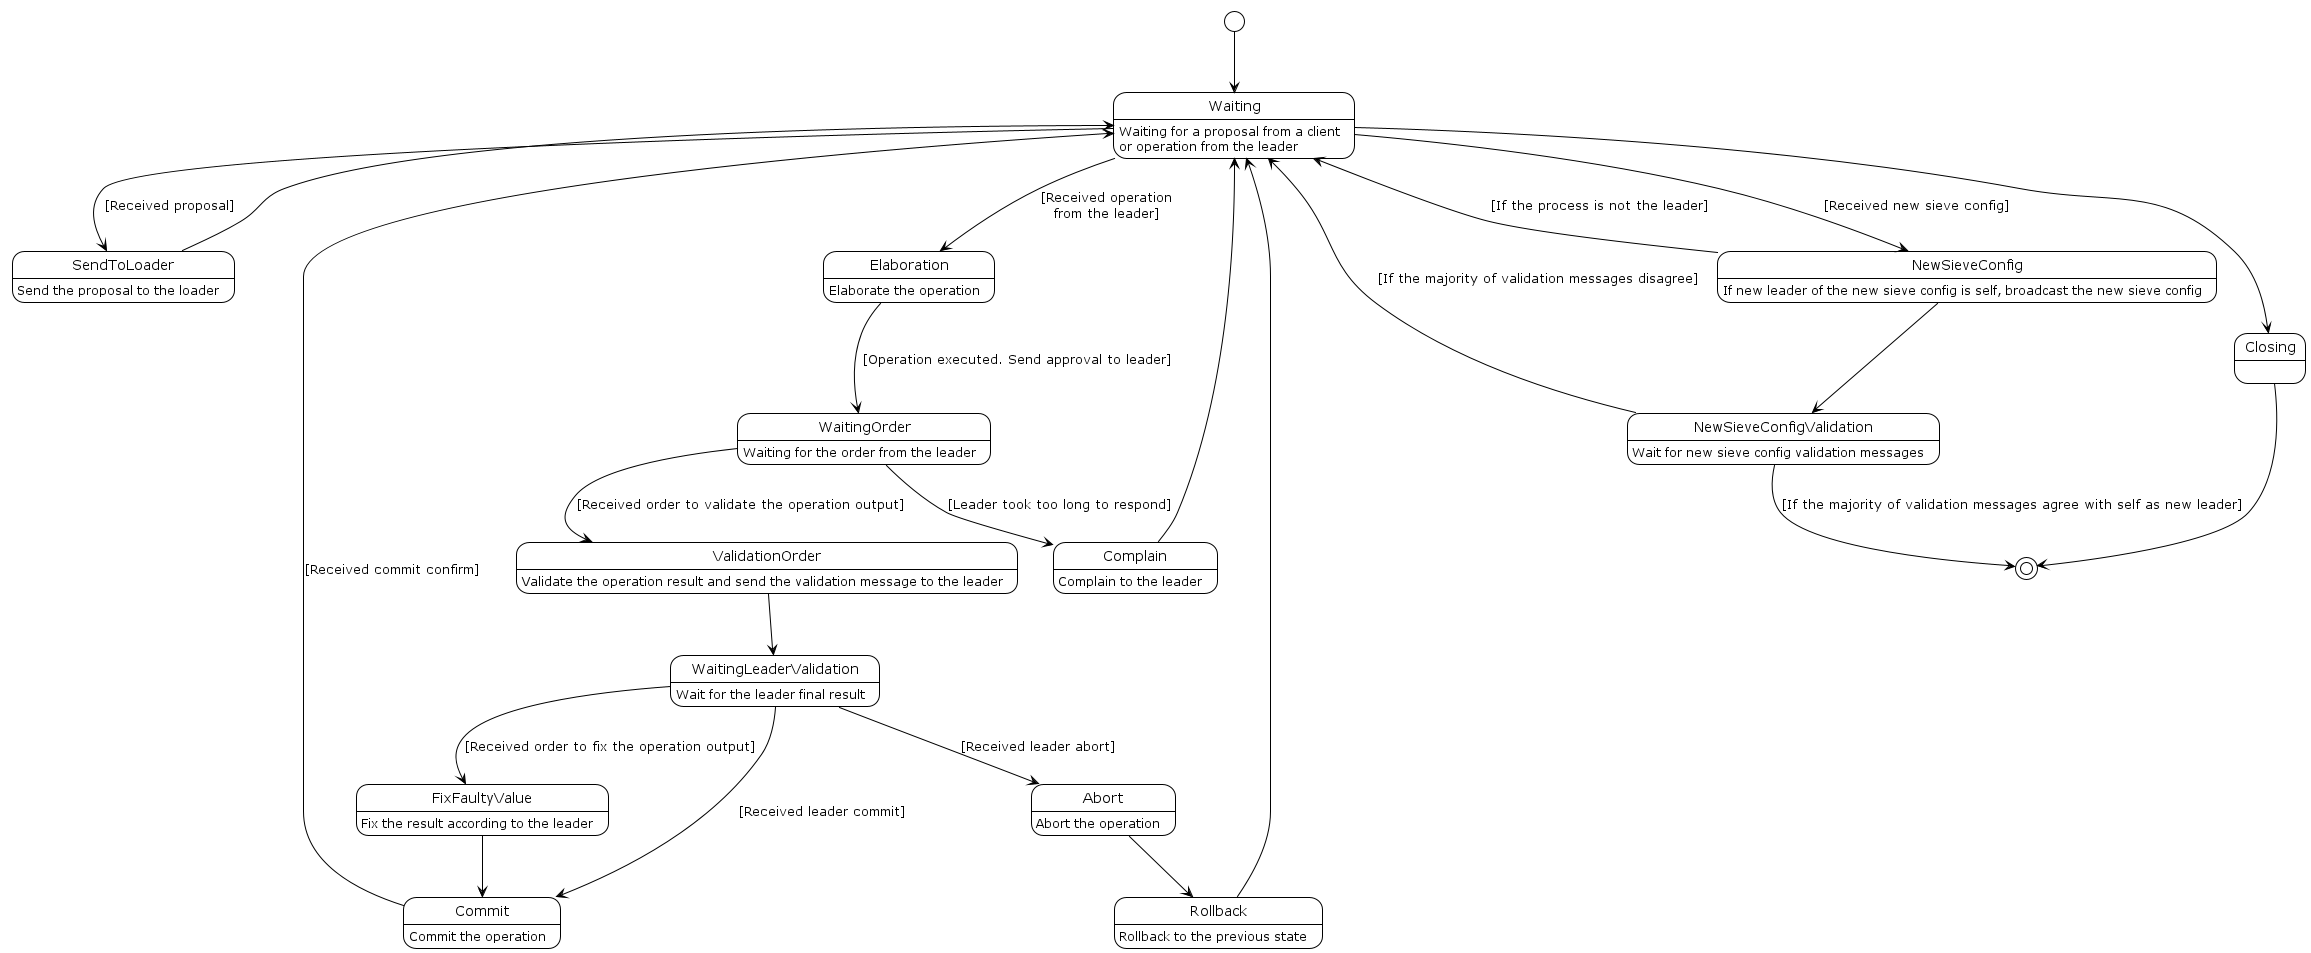
\includegraphics[width=1\linewidth]{figures/slave.png}
    \caption{State diagram of non-leaders nodes}
    \label{fig:slave}
\end{figure}

\begin{itemize}
    \item \textbf{Waiting}
    
    In this state, the slave waits for proposals from a client or operations from the leader.

    \item \textbf{SendToLeader}
    
    If the process receives a proposal from a client, it forwards the proposal to the leader.
    
    \item \textbf{Elaboration}
    
    Upon receiving an execute operation message from the leader, the process elaborates on the operation sent by the leader.
    
    \item \textbf{WaitingOrder}
    
    After completing the operation, the process sends the result to the leader and awaits the next instruction. If there's a delay in the leader's response, the process transitions to the \textbf{Complain} state.
    
    \begin{itemize}
        \item \textit{Complain}
        
        The process sends a complaint to the leader and transitions back to the \textbf{Waiting} state.
    \end{itemize}
    
    \item \textbf{ValidationOrder}
    
    Upon receiving the leader's results, the process validates the result, using a validation predicate, and sends a validation message.
    
    \item \textbf{WaitingLeaderValidation}
    
    The process waits for the final message from the leader.
    
    \begin{itemize}
        \item \textit{Commit}
        
        If the process receives a commit message, it commits the operation and transitions back to the \textbf{Waiting} state.
        
        \item \textit{FixFaultyValue}
        
        Upon receiving a correction message, the process updates the result and transitions to the \textbf{Commit} state.
        
        \item \textit{Abort}
        
        If the process receives an abort message, it aborts the current operation and transitions to the \textbf{Rollback} state.
        
    \end{itemize}
    
    \item \textbf{Rollback}
    
    The process rolls back to the previous correct state.
    
    \item \textbf{NewSieveConfig}
    
    Upon receiving the new sieve configuration, if the process is the new leader, it broadcasts the new configuration to other processes; otherwise, it returns to the \textbf{Waiting} state.
    
    \item \textbf{NewSieveConfigValidation}
    
    The process waits for validation messages regarding the new sieve configuration. If the majority agrees, this process becomes a leader.
    
    \item \textbf{Closing}
    
    Upon receiving a close message, the process shuts down.
    
\end{itemize}


\subsubsection{Network}

\begin{figure}[H]
    \centering
    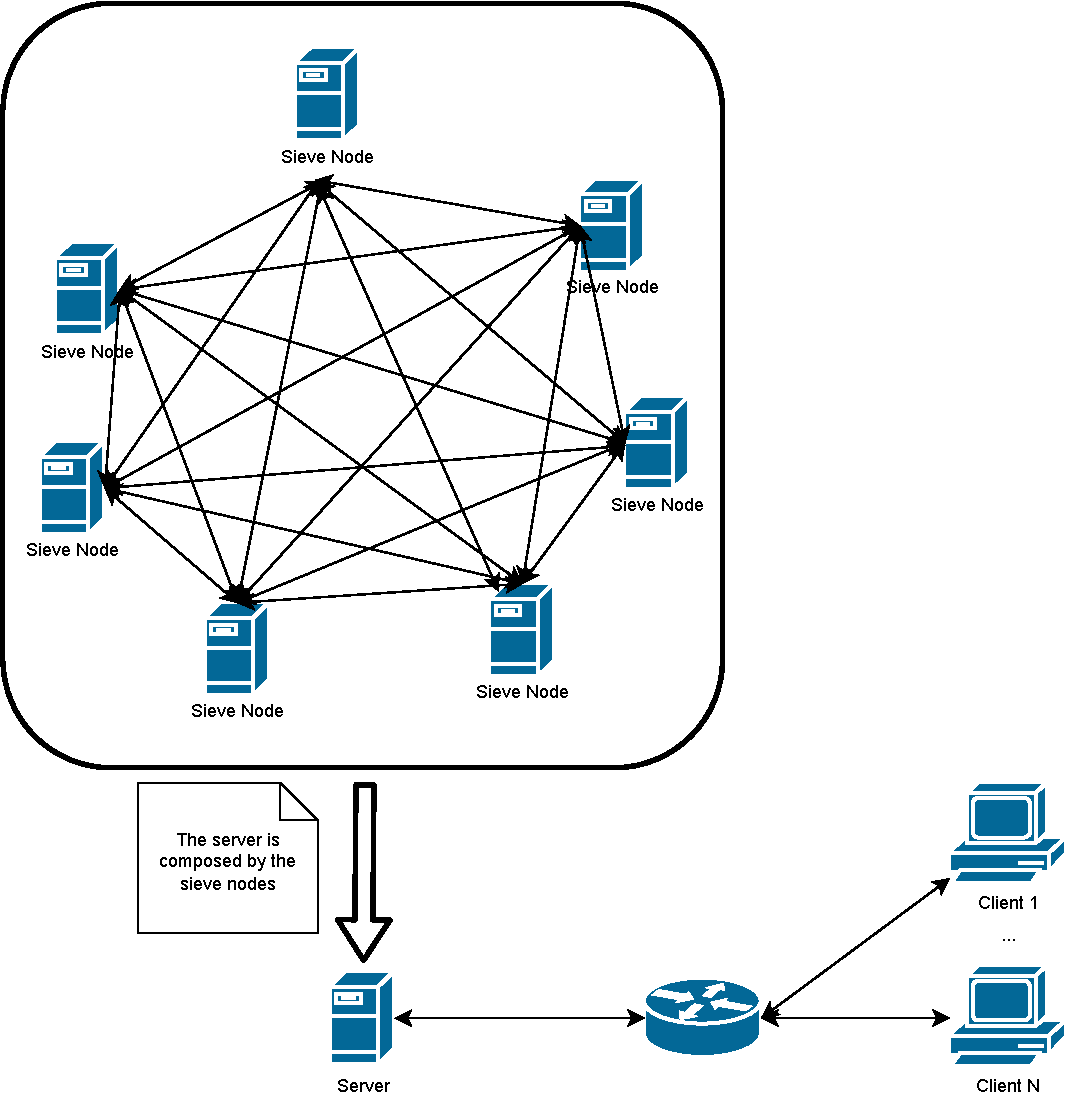
\includegraphics[width=1\linewidth]{figures/network.pdf}
    \caption{Logic representation of the network used in our simulation.}
    \label{fig:network}
\end{figure}

The behavior of all nodes in the network, while the number of nodes is indefinite, manifests as a single unified server responsible for receiving, processing requests, and sending responses to the client. This is achieved through the centralized management depicted in figures \ref{fig:leader} and \ref{fig:slave}. Most queries in this configuration go through the leader node. Because of the RSM's nature, any slave process that receives a request is redirected to the current leader to be handled, with the exception of requests for values given keys, which can be handled by any node.

\section{Implementation Details}

In the development of the Sieve protocol simulation, several noteworthy implementation details have been incorporated to enhance the robustness and effectiveness of the software. The documentation for this project is crafted using \href{https://www.mkdocs.org/}{\textit{mkdocs}}, providing a structured and accessible resource for understanding the intricacies of the implemented solution.

Here are some salient implementation details of the project:

\begin{itemize}
    \item To emulate real-world scenarios and Byzantine faults, the simulation incorporates dynamic node behavior. Nodes can exhibit various forms of Byzantine behavior, such as sending conflicting messages or intentionally delaying message propagation. This dynamic simulation enriches the testing environment and ensures a more comprehensive evaluation of the Sieve protocol's effectiveness.
    \item Cryptographic techniques play a pivotal role in the Sieve protocol's functionality. The implementation includes the integration of cryptographic libraries to secure communication channels and validate the integrity of messages exchanged between nodes. This cryptographic layer enhances the overall security posture of the system.
    \item The Sieve protocol's consensus algorithm has been adapted to accommodate the dynamic nature of Byzantine faults. The algorithm dynamically adjusts its parameters to respond to changes in the network's behavior, allowing for a more adaptive and resilient consensus-building process, the total number of the nodes must be at least 3f + 1, where f is the number of faulty nodes.
    \item The simulation logs events and interactions at various stages of the protocol execution. This logging serves as a valuable resource for simulation analysis, enabling the identification of patterns, bottlenecks, and potential improvements in the Sieve protocol's performance.
\end{itemize}

Aiming to simplify our implementation, it was also decided:

\begin{itemize}
    \item not to allow changes to the cluster (addition/removal of processes) while the RSM is already in execution;
    \item not to maintain the execution data and logs after the RSM shutdown. This implies that there are always nodes with base configurations at restart, without memory of the previous states and events.
\end{itemize}

Given the complexity of the Sieve protocol and the nuanced challenges posed by Byzantine faults, these implementation details collectively contribute to a simulation environment. The accompanying mkdocs documentation further provides a structured guide for users and developers, facilitating a smooth understanding of the software artifacts.

\section{Self-assessment / Validation}

It was necessary to conduct a variety of tests with varying degrees of detail and emphasis on various areas to confirm that the software developed was accurate. The following subsection contains an account of the parts that were tested using autonomous testing. Additionally, manual testing was done, in particular to evaluate the GUI and particular client-server interaction.

\subsection{Sieve protocol testing}
The \textbf{unittest} package, a Python framework for test-driven development and code correctness verification, was utilized to confirm in greater detail the correct functionality of the Sieve components (tests results can be found in Figure \ref{fig:tests}).

All tests created use one or more instances of the client to verify the correctness of various features. The client instance is necessary to send operations requests, as well as checking the responses and log messages received.

A system of "debug messages" was developed in order to dynamically configure internal parameters of the Sieve processes, ensuring test reproducibility.

In particular, the following tests were performed, which can be found within the file \textit{src/test.py}:

\begin{itemize}
    \item \textbf{Base functionalities}

        To verify that a Sieve process's primary capabilities were correct, the following tests were conducted:
        \begin{itemize}
            \item \textbf{test\_commit}: tests if the commit section is executed
            \item \textbf{test\_abort}: tests if the abort section is executed
            \item \textbf{test\_rollback}: tests if the rollback section is executed
            \item \textbf{test\_complain}: tests if a complain occurs
            \item \textbf{test\_new\_sieve\_config\_after\_abort}: tests if a new sieve config starts after an abort
            \item \textbf{test\_new\_sieve\_config\_after\_complain}: tests if a new sieve config starts after a complaint
            \item \textbf{test\_close}: tests if the Sieve processes stop when reaching the close message
        \end{itemize}

    \item \textbf{Functionalities combinations}
    
        At this point are listed the tests for compound and serialized operations:
        \begin{itemize}
            \item \textbf{test\_multiple\_commit}: tests if multiple commits are executed correctly
            \item \textbf{test\_commit\_after\_new\_sieve\_config}: tests if the commit section is executed after a new sieve config, so if a new leader executes it
            \item \textbf{test\_not\_queued\_operation}: tests if, after a new sieve config, the new leader has an empty operation queue if the previous leader has it in turn
            \item \textbf{test\_commit\_node\_queued\_operation}: tests if, after a new sieve config, the new leader has an operation queue with the operations not executed by the previous leader
            \item \textbf{test\_two\_clients\_commit}: tests the commit of operations sent by more than a single client
        \end{itemize}

    \item \textbf{Values requests}
    
        The tests below were used to check if the functionalities offered to the client are correct:
        \begin{itemize}
            \item \textbf{test\_request\_non\_existing\_value}: tests the case when a client requests a value associated with a non-existing key
            \item \textbf{test\_request\_existing\_value}: tests the case when a client requests a value associated with an existing key
            \item \textbf{test\_request\_non\_existing\_value\_after\_abort}: tests the case when a client requests a value associated with a non-existing key because the abortion of the relative operation which should have added the key-value
            \item \textbf{test\_request\_existing\_value\_after\_abort}: tests the case when a client requests a value associated with an existing key, which must exist also if another operation aborts
            \item \textbf{test\_request\_existing\_value\_all}: tests the proper functioning of consensus
        \end{itemize}
    
\end{itemize}

\begin{figure}[H]
    \centering
    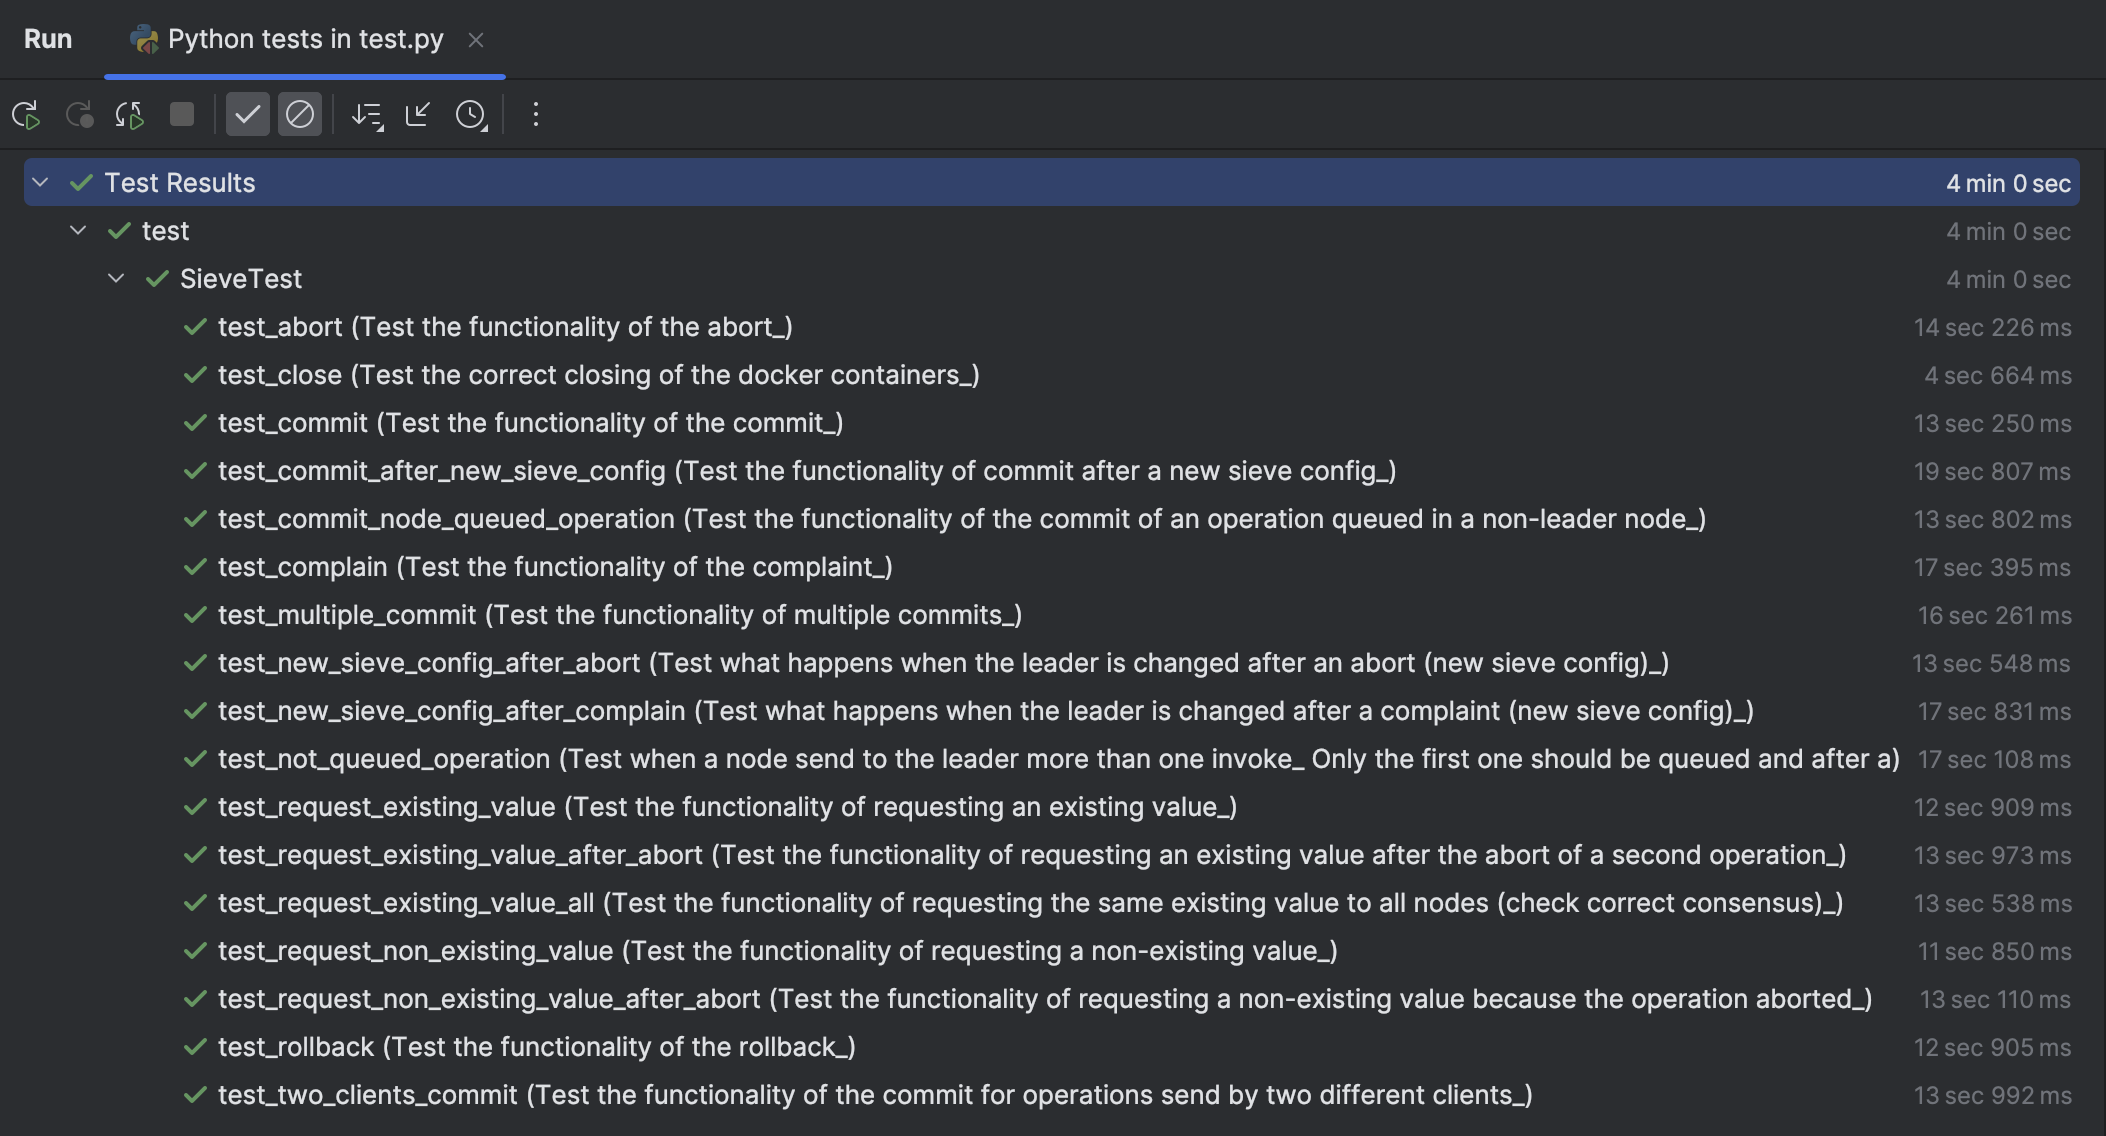
\includegraphics[width=.9\linewidth]{figures/tests.png}
    \caption{Screenshot of executed tests results.}
    \label{fig:tests} 
\end{figure}


\section{Deployment Instructions}

To ensure a smooth deployment of the software in a clean environment, follow these steps:

\subsection{Prerequisites}

Ensure that the following prerequisites are installed on the target system:

\begin{itemize}
    \item \textbf{Python 3.10}: Install Python 3.10 on the system. You can download the target version from the \href{https://www.python.org/downloads/}{official Python website}.

    \item \textbf{pip}: Ensure that the Python package installer, pip, is available. It is typically installed automatically with Python. If not, install it using the appropriate package manager for your system.

    \item \textbf{Docker}: Install Docker to enable containerization. Follow the instructions for your operating system on the \href{https://docs.docker.com/get-docker/}{official Docker website}.

\end{itemize}

\subsection{Deployment Steps}

Follow these steps to deploy and launch the software:

\begin{enumerate}
    \item \textbf{Clone the Repository}
    
    Clone the project repository to the target system using Git:
    
    \begin{verbatim}
    git clone https://dvcs.apice.unibo.it/pika-lab/courses/ds/projects/
    ds-project-detuglie-artegiani-grateron-ay2324.git
    
    cd ds-project-detuglie-artegiani-grateron-ay2324
    \end{verbatim}

    \item \textbf{Install Python Dependencies}
    
    Install the required Python dependencies listed in the \textit{requirements.txt }file:

    \begin{verbatim}
    pip install -r requirements.txt
    \end{verbatim}

    \item \textbf{Build Docker Image}
    
    Build the Docker image for the project. Ensure that Docker is running, then execute the following command from the project root:

    \begin{verbatim}
    docker build -t sieve-process .
    \end{verbatim}

    \item \textbf{Run The Application}
    
    Run the application with the following command:

    \begin{verbatim}
    python3 ./src/client.py
    \end{verbatim}

\end{enumerate}

These steps assume a clean environment and provide the necessary instructions for setting up and deploying the software with minimal configuration. These details are also available in the project's \textit{README}.

If the client cannot communicate with the containers it can be required to add them in \textit{/etc/hosts} file using the following sintax:

    \begin{verbatim}
    127.0.0.1 process1
    ...
    127.0.0.1 processN
    \end{verbatim}

\subsection{Build documentation}

Follow these steps to build the documentation as a web page:

\begin{enumerate}
   \item \textbf{Install MkDocs}
   
   Install MkDocs and his dependency using the following command:

   \begin{verbatim}
       pip install -r ./mkdocs/requirements.txt
   \end{verbatim}

   \item \textbf{Build the documentation}
   
   Generate web page:

   \begin{verbatim}
       mkdocs build
   \end{verbatim}

   \item \textbf{Consult documentation}
   
   It is possible to self-host and view the documentation with the following command:

   \begin{verbatim}
       mkdocs serve
   \end{verbatim}

\end{enumerate}


For more information check the \href{https://www.mkdocs.org/user-guide/}{MkDocs documentation}.

\section{Usage Examples}

Once the \textit{src/client.py} script is executed, it will launch the following GUI, as illustrated in Figure \ref{fig:gui}.

\begin{figure}[H]
    \centering
    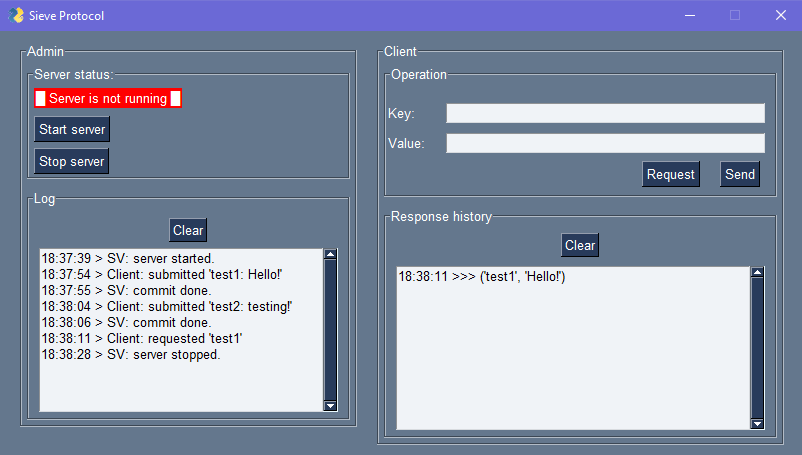
\includegraphics[width=.9\linewidth]{figures/gui.png}
    \caption{Interface for controlling the application}
    \label{fig:gui} 
\end{figure}

To begin, click the "Start Server" button to initiate the server. The "Log" field provides real-time updates on the status of the operations.

After the server has been started, operations, to update the shared dictionary, can be sent for execution by entering a key-value pair and clicking the "Send" button. Alternatively, clicking the "Request" button will query the value associated with the entered key. The responses to these actions are displayed in the "Response history" section.
The server can be stopped at any time by clicking the "Stop Server" button.

This interface provides a straightforward means of interacting with the application, allowing users to manage operations and monitor responses conveniently.

\section{Conclusions}

In conclusion, this project not only achieved the successful implementation and simulation of the Sieve protocol but also made us practice the theoretical aspects we learned during the course.
Summarizing the activities we did, we started studying the Sieve protocol from the paper \cite{paper} and the connected documentation, and then we analyzed and extrapolated the implementation aspects we used for the design phase. After the design phase, we focused on the implementation and deployment. We opted for the use of \textit{Docker} to create a cluster of Sieve processes and the use of \textit{Python DGRAM sockets} for the communication. The group tried as much as possible to comply with the test-driven development approach using \textit{unittest} framework. In the first part testing was concentrated on base functionalities, then on routines and simulation of some more complex scenarios. 

\subsection{Future Works}

In this work, we have developed a representation of the Sieve Protocol in Python, focusing on its behavior and interaction within a distributed network. However, several aspects have not been addressed or could be further improved:

\begin{itemize}
    \item \textbf{Greater Fault Tolerance}
    
    Although the protocol includes mechanisms for leader election and failure recovery, further analysis and testing are needed to assess its robustness in various failure scenarios, such as denial-of-service attacks.
    
    \item \textbf{Database Integration}
    
    Currently, our implementation relies on a shared dictionary for storing data. In future work, we aim to integrate a more robust data storage solution, such as a distributed database or a blockchain, to enhance data persistence and reliability.

    \item \textbf{Performance improvement}

    Currently, each Sieve process does its tasks using three threads without any special optimizations. Further research could benefit from using additional thread-specific data types and instructions to improve performance.
    
    \item \textbf{User Interface Enhancements}
    
    While we have implemented a basic client interface for interacting with the network, there is room for improvement in usability and functionality. Future work could involve refining the user interface to provide users with more intuitive controls and informative feedback.

    \item \textbf{Real-scenario implementation}

    For the time being, this project only offers a localhost simulation. However, future work could expand this implementation of the Sieve protocol to a real-world setting, i.e., a distributed system that is available via the internet.
\end{itemize}

Addressing these areas of improvement would not only enhance the functionality and performance of the Sieve Protocol implementation but also contribute to the broader understanding of distributed consensus protocols.

\newpage

\subsection{What Did We Learn}

Throughout the development of this project, several key learnings were acquired:

\begin{itemize}
    \item \textbf{Docker Utilization}
    
    The project provided hands-on experience in using Docker for containerization. Understanding how to create, deploy, and manage Docker containers proved to be crucial for achieving a scalable and consistent simulation environment.

    \item \textbf{Inter-Container Communication}
    
    The project involved making Docker containers communicate with each other using Python sockets. This learning extended to managing communication channels between distributed nodes, a valuable skill in the context of distributed systems.

    \item \textbf{PySimpleGUI for GUI Development}
    
    Integration of PySimpleGUI for creating the GUI enhanced the understanding of developing user-friendly interfaces in Python. This knowledge is transferable to various application domains requiring interactive user interactions.

    \item \textbf{Automated Testing with unittest}
    
    The use of the unittest framework in Python for automated testing contributed to the development of robust and reliable code. Implementing test cases and ensuring code coverage became integral to maintaining software quality.

    \item \textbf{Processes Synchronization}

    It was required to learn how to synchronize the states and actions of individual processes in order to synchronize the various stages of the Sieve protocol.

    \item \textbf{Consistency and Consensus}

    Understanding consistency and consensus is necessary since putting the Sieve protocol into practice.

    \item \textbf{Byzantine Fault Tolerance Concepts}
    
    Working on the Sieve protocol simulation deepened the understanding of Byzantine fault tolerance concepts in distributed systems. Practical implementation and experimentation illuminated the challenges and solutions associated with mitigating malicious behaviors.

\end{itemize}

These learnings collectively contribute to a well-rounded skill set, encompassing containerization, inter-container communication, GUI development, automated testing, and distributed systems concepts. The insights gained are not only applicable to this project but also lay a foundation for addressing challenges in diverse software development scenarios.



\nocite{*} % Includes all references from the `references.bib` file
\bibliographystyle{plain}
\bibliography{references}

\end{document}
